% old figure environments



% Figures~\ref{fig:moduloPlot_60h}--\ref{fig:moduloPlot_Endgame} show results for single random seed results to calorimeter sum data for the four datasets. 

% \begin{figure}[]
%     \centering
%     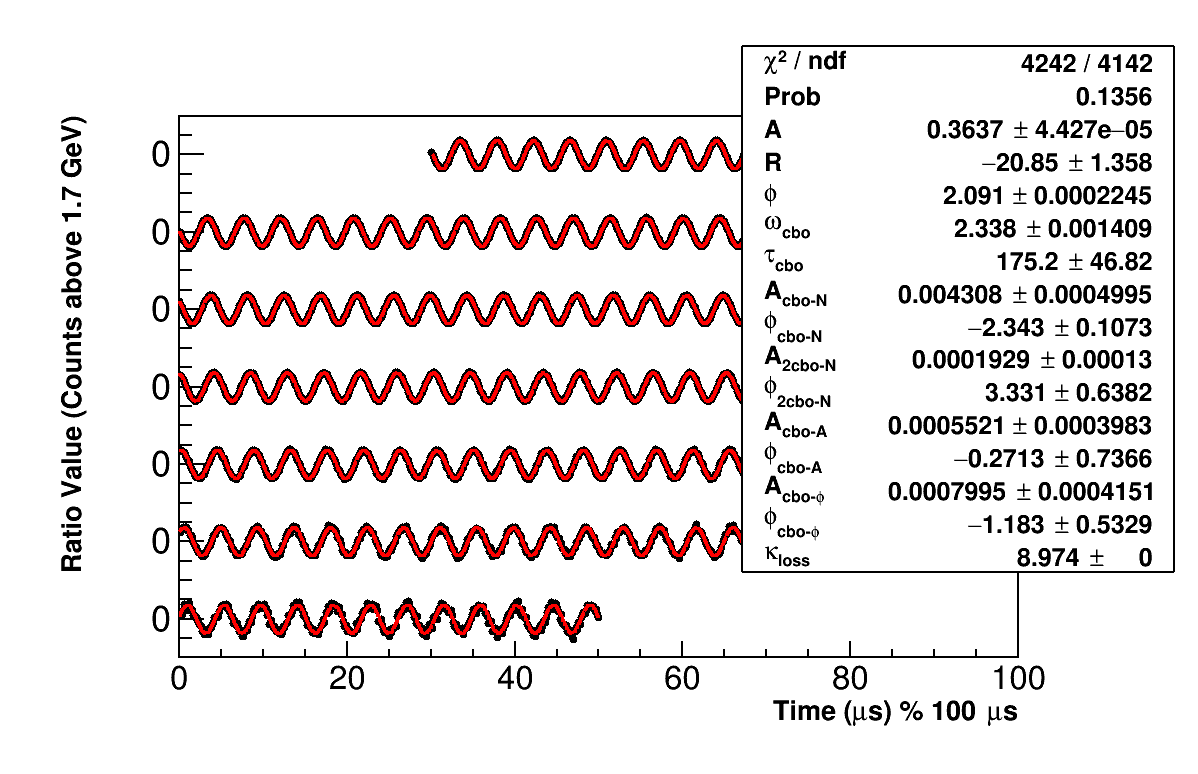
\includegraphics[width=.8\textwidth]{fullRatio_moduloPlot_60h}
%     \caption[60h dataset calorimter sum fit result]{Single random seed fit result to calorimeter sum of 60h dataset. The x axis is in units of \mus{} modulo \mus{100}, with successive portions of the data points and fit shifted downwards on the plot. The fit ranges from 30.2--\mus{650}.}
%     \label{fig:moduloPlot_60h}
% \end{figure}

% \begin{figure}[]
%     \centering
%     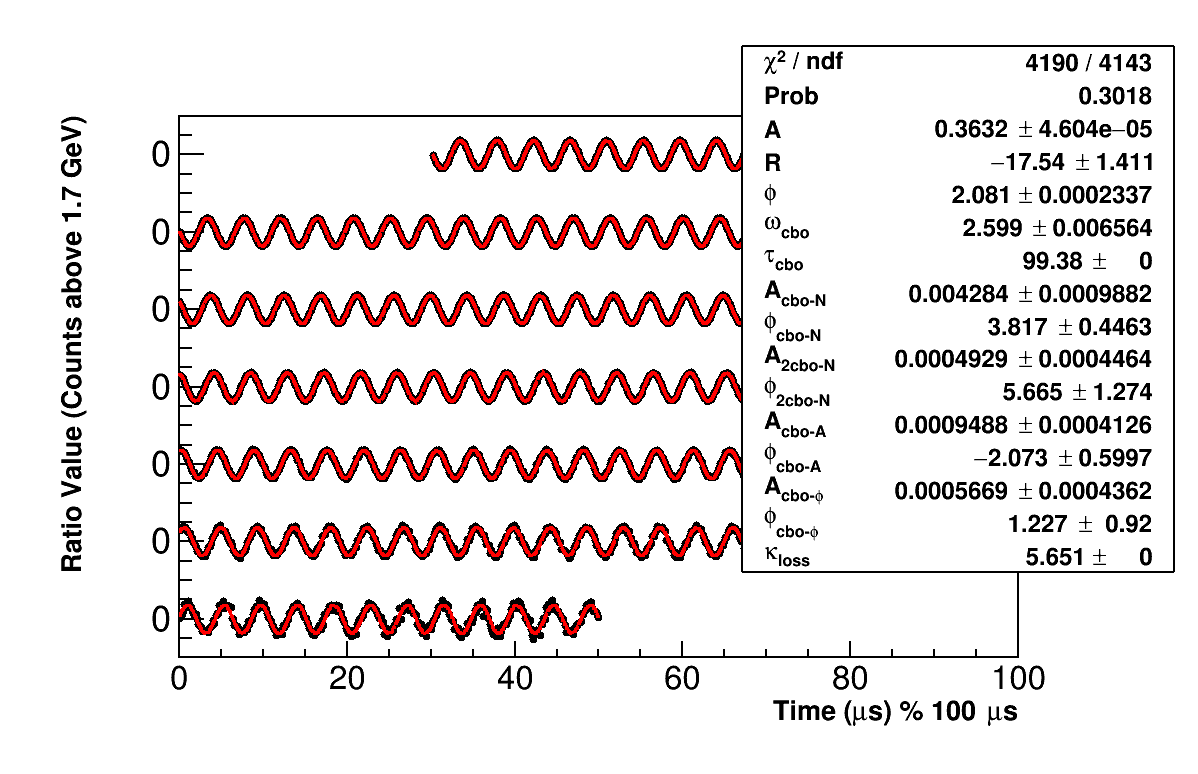
\includegraphics[width=.8\textwidth]{fullRatio_moduloPlot_HighKick}
%     \caption[HighKick dataset calorimter sum fit result]{Single random seed fit result to calorimeter sum of HighKick dataset. The x axis is in units of \mus{} modulo \mus{100}, with successive portions of the data points and fit shifted downwards on the plot. The fit ranges from 30.2--\mus{650}.}
%     \label{fig:moduloPlot_HighKick}
% \end{figure}

% \begin{figure}[]
%     \centering
%     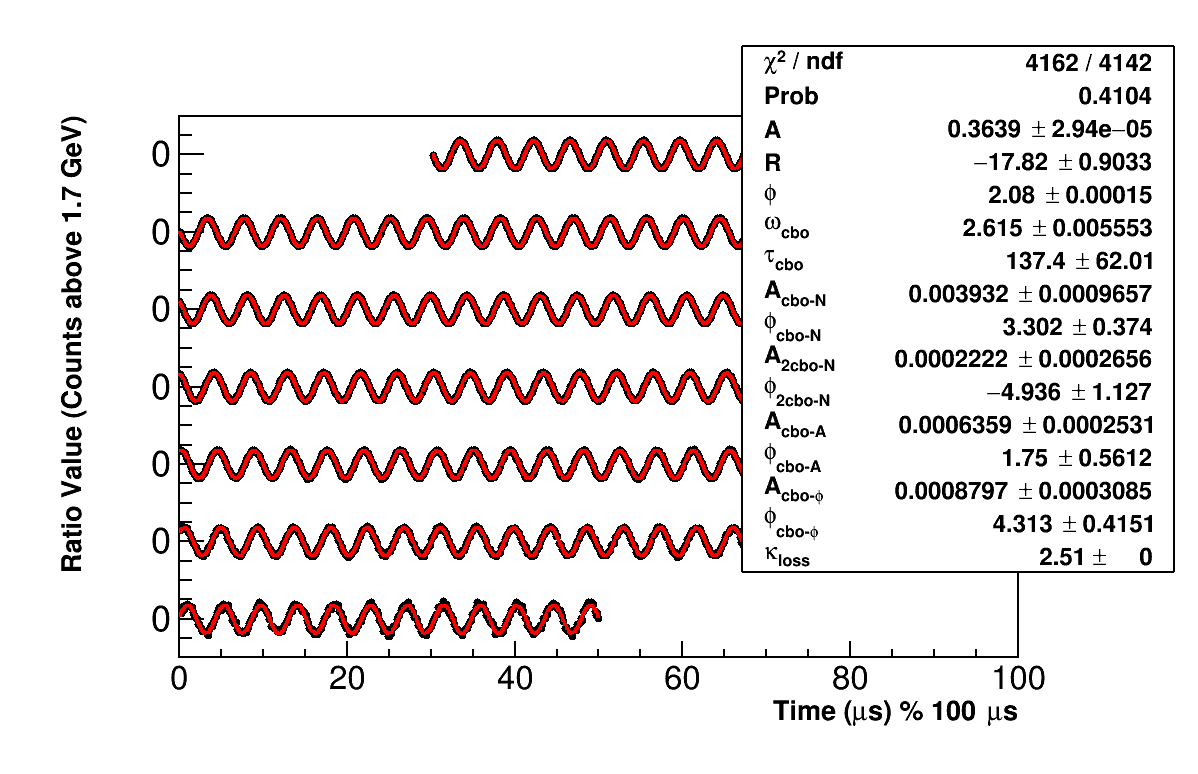
\includegraphics[width=.8\textwidth]{fullRatio_moduloPlot_9d}
%     \caption[9d dataset calorimter sum fit result]{Single random seed fit result to calorimeter sum of 9d dataset. The x axis is in units of \mus{} modulo \mus{100}, with successive portions of the data points and fit shifted downwards on the plot. The fit ranges from 30.2--\mus{650}.}
%     \label{fig:moduloPlot_9d}
% \end{figure}

% \begin{figure}[]
%     \centering
%     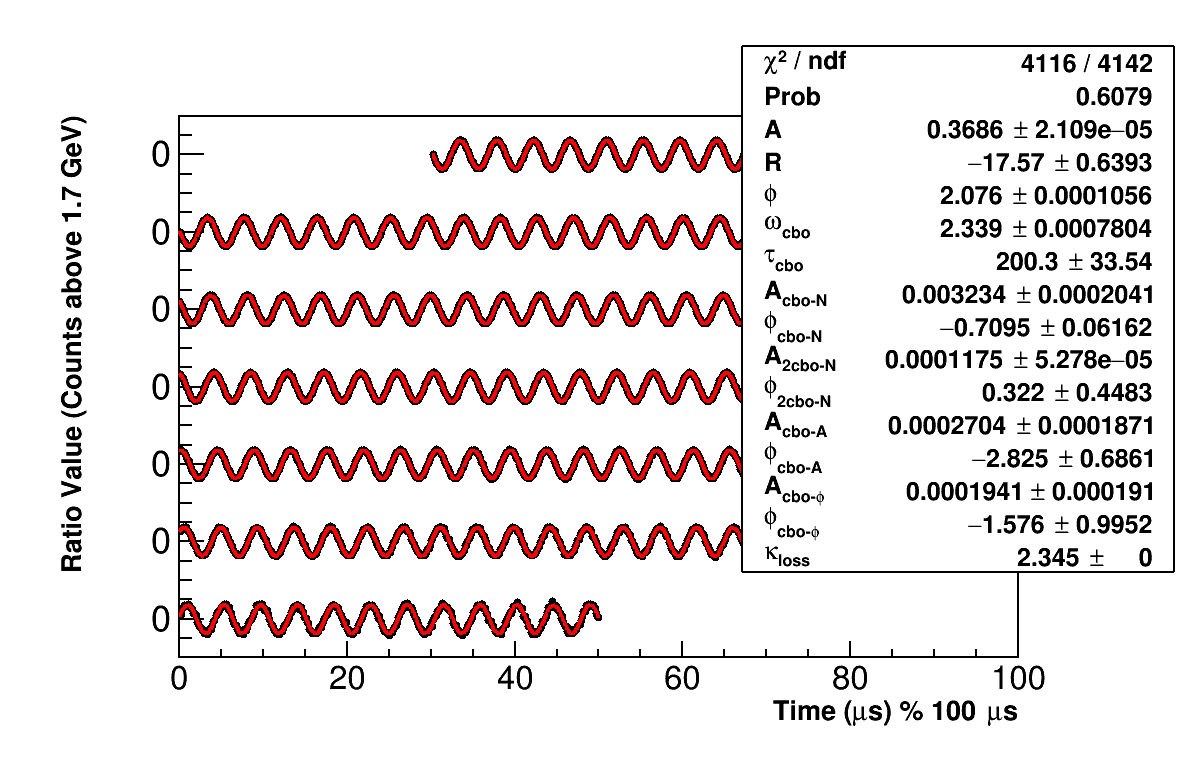
\includegraphics[width=.8\textwidth]{fullRatio_moduloPlot_Endgame}
%     \caption[Endgame dataset calorimter sum fit result]{Single random seed fit result to calorimeter sum of Endgame dataset. The x axis is in units of \mus{} modulo \mus{100}, with successive portions of the data points and fit shifted downwards on the plot. The fit ranges from 30.2--\mus{650}.}
%     \label{fig:moduloPlot_Endgame}
% \end{figure}





% \begin{figure}[]
% \centering
%     \begin{subfigure}[]{0.45\textwidth}
%         \centering
%         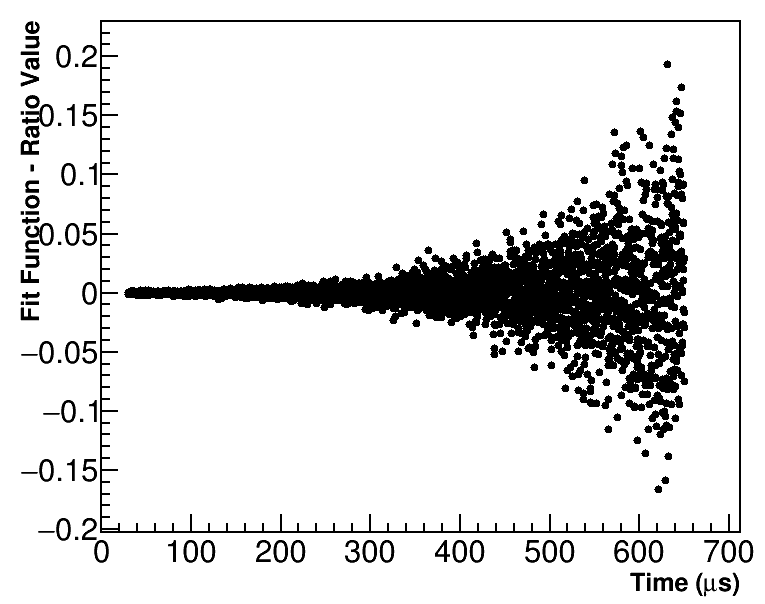
\includegraphics[width=\textwidth]{fitResidual_60h}
%         \caption{Fit residuals.}
%     \end{subfigure}
%     \begin{subfigure}[]{0.45\textwidth}
%         \centering
%         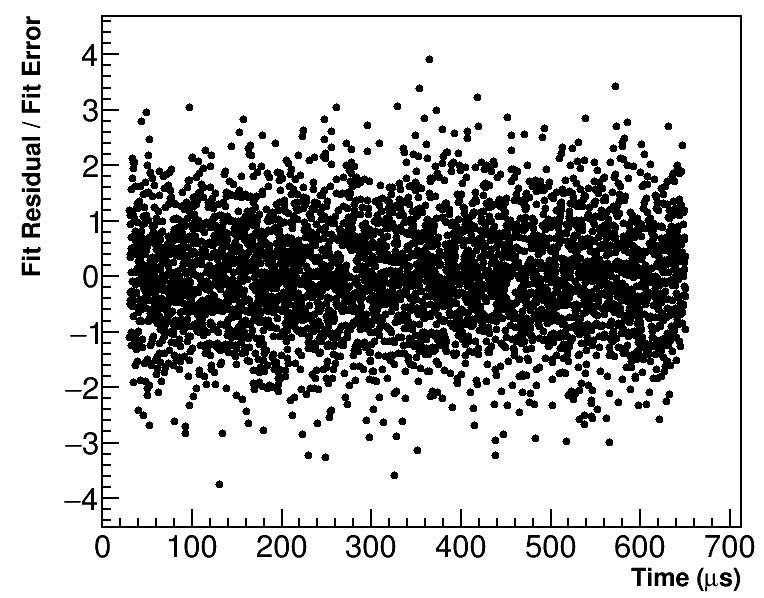
\includegraphics[width=\textwidth]{fitPull_60h}
%         \caption{Fit pulls.}
%     \end{subfigure}% %you need this % here to add spacing between subfigures
%     \vspace{4mm}
%     \begin{subfigure}[]{0.5\textwidth}
%         \centering
%         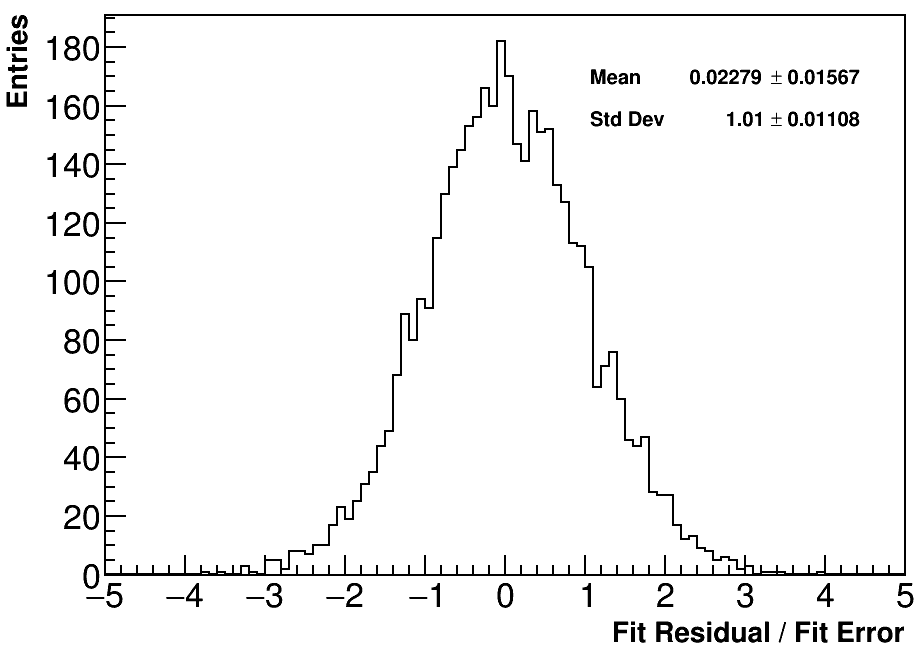
\includegraphics[width=\textwidth]{fitPull_projected_60h}
%         \caption{Fit pulls projected onto the y axis. Note the Gaussian shape centered around 0 with unit width.}
%     \end{subfigure}
% \caption[Residuals and pulls for the ratio fit to the 60h dataset]{Residuals and pulls for the ratio fit to the 60h dataset. There is no obvious structure in any of the plots.}
% \label{fig:fitResiduals_60h}
% \end{figure}

% \begin{figure}[]
%     \centering
%     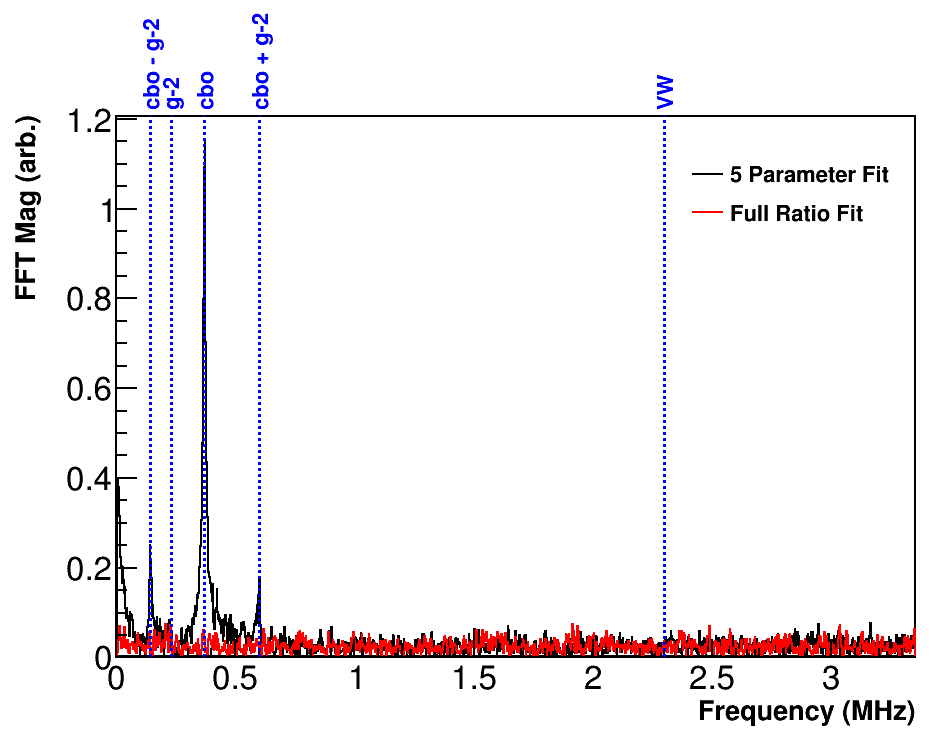
\includegraphics[width=0.6\textwidth]{FFTComparison_FullRatio_60h}
%     \caption[FFT of the 60h dataset fit residuals]{FFT of the 60h dataset fit residuals compared to the fit residuals from a 5 parameter fit to the data. All peaks have been eliminated above the noise.}
%     \label{fig:FFT_60h}
% \end{figure}




\begin{landscape}
\begin{figure}[]
% \centering
\begin{minipage}[t]{0.48\linewidth}
    \begin{subfigure}[]{0.5\linewidth}
        \centering
        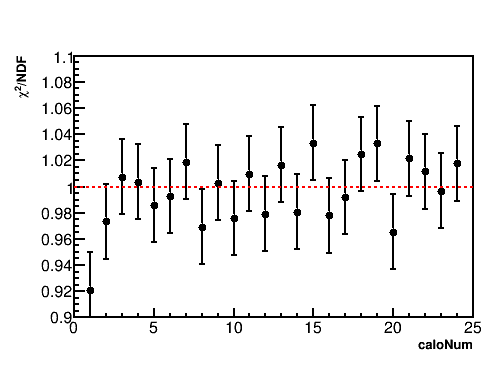
\includegraphics[width=\linewidth]{FullRatioFit_Chi2NDF_Vs_Calo_Canv_60h}
        \caption{60h dataset.}
    \end{subfigure}% %you need this % here to add spacing between subfigures
    \begin{subfigure}[]{0.5\linewidth}
        \centering
        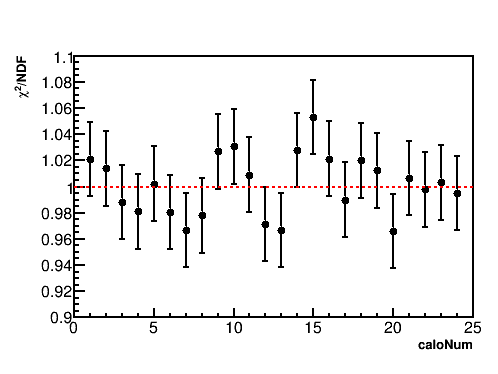
\includegraphics[width=\linewidth]{FullRatioFit_Chi2NDF_Vs_Calo_Canv_HighKick}
        \caption{HighKick dataset.}
    \end{subfigure}

    \begin{subfigure}[]{0.5\linewidth}
        \centering
        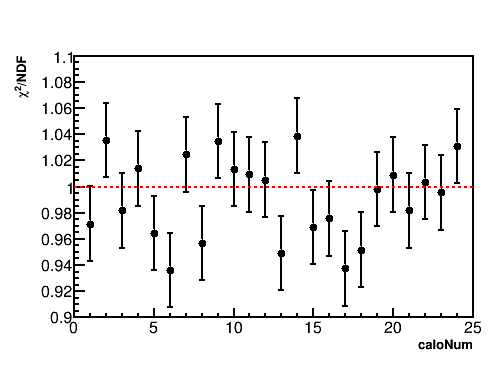
\includegraphics[width=\linewidth]{FullRatioFit_Chi2NDF_Vs_Calo_Canv_9d}
        \caption{9d dataset.}
    \end{subfigure}% %you need this % here to add spacing between subfigures
    \begin{subfigure}[]{0.5\linewidth}
        \centering
        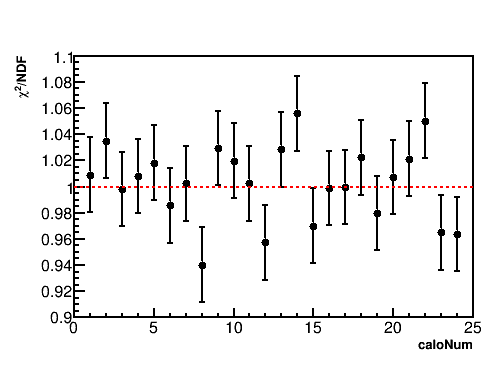
\includegraphics[width=\linewidth]{FullRatioFit_Chi2NDF_Vs_Calo_Canv_Endgame}
        \caption{Endgame dataset.}
    \end{subfigure}
\captionsetup{width=0.9\linewidth}
\caption[\chisq/NDF versus calorimeter number]{\chisq/NDF versus calorimter for the Run~1 precession frequency analysis datasets.}
\label{fig:caloFits_chi2}
% \end{figure}

\end{minipage}
\hfill
\begin{minipage}[t]{0.48\linewidth}

% \begin{figure}[]
% \centering
    \begin{subfigure}[]{0.5\linewidth}
        \centering
        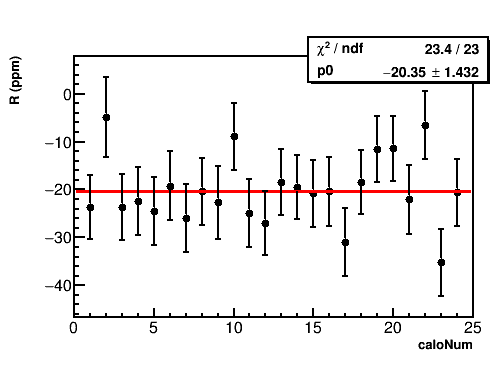
\includegraphics[width=\linewidth]{FullRatioFit_R_Vs_Calo_Canv_60h}
        \caption{60h dataset.}
    \end{subfigure}% %you need this % here to add spacing between subfigures
    \begin{subfigure}[]{0.5\linewidth}
        \centering
        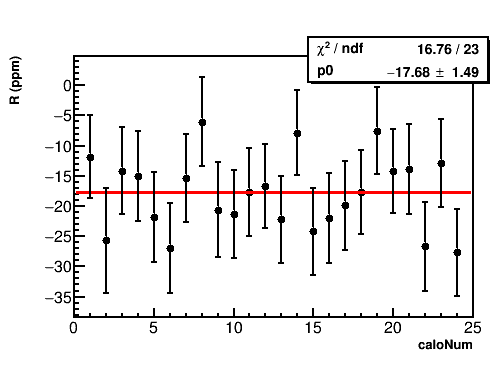
\includegraphics[width=\linewidth]{FullRatioFit_R_Vs_Calo_Canv_HighKick}
        \caption{HighKick dataset.}
    \end{subfigure}

    \begin{subfigure}[]{0.5\linewidth}
        \centering
        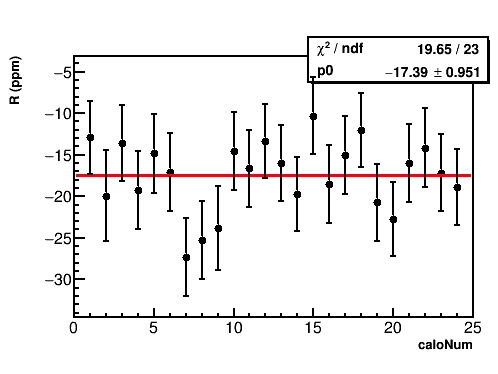
\includegraphics[width=\linewidth]{FullRatioFit_R_Vs_Calo_Canv_9d}
        \caption{9d dataset.}
    \end{subfigure}% %you need this % here to add spacing between subfigures
    \begin{subfigure}[]{0.5\linewidth}
        \centering
        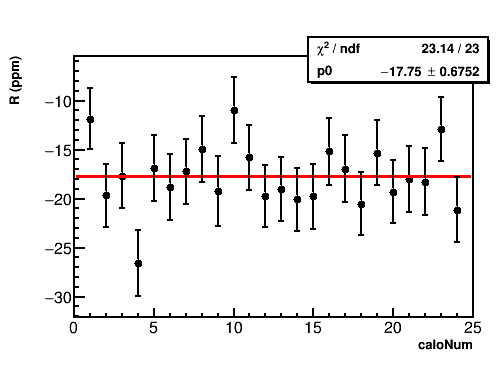
\includegraphics[width=\linewidth]{FullRatioFit_R_Vs_Calo_Canv_Endgame}
        \caption{Endgame dataset.}
    \end{subfigure}
\captionsetup{width=0.9\linewidth}
\caption[$R$ versus calorimeter number]{$R$ versus calorimter for the Run~1 precession frequency analysis datasets. A straight line fit was performed on the fitted values, with the fit result shown in the upper right box as parameter $p_{1}$ in units of ppm.}
\label{fig:caloFits_R}
\end{minipage}
\end{figure}
\end{landscape}








% \begin{figure}[]
% \centering
%     \begin{subfigure}[]{0.45\textwidth}
%         \centering
%         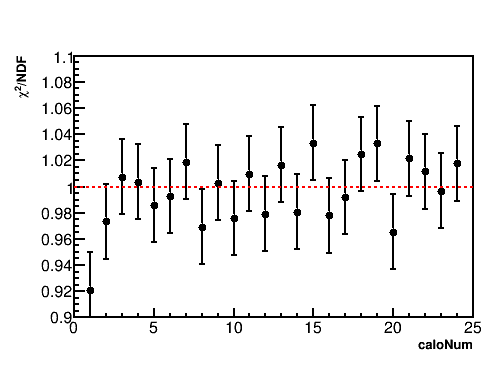
\includegraphics[width=\textwidth]{FullRatioFit_Chi2NDF_Vs_Calo_Canv_60h}
%         \caption{60h dataset.}
%     \end{subfigure}% %you need this % here to add spacing between subfigures
%     \begin{subfigure}[]{0.45\textwidth}
%         \centering
%         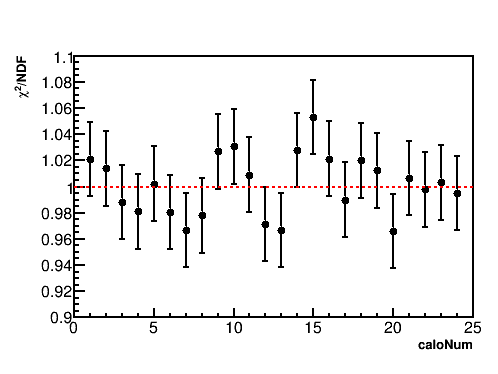
\includegraphics[width=\textwidth]{FullRatioFit_Chi2NDF_Vs_Calo_Canv_HighKick}
%         \caption{HighKick dataset.}
%     \end{subfigure}

%     \begin{subfigure}[]{0.45\textwidth}
%         \centering
%         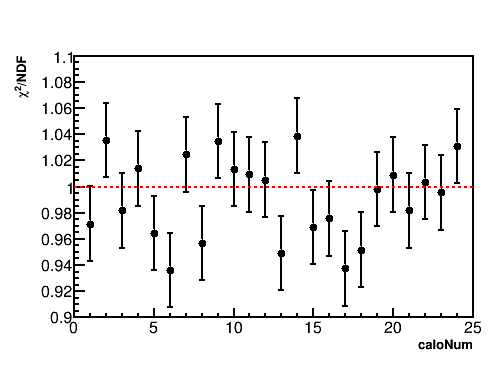
\includegraphics[width=\textwidth]{FullRatioFit_Chi2NDF_Vs_Calo_Canv_9d}
%         \caption{9d dataset.}
%     \end{subfigure}% %you need this % here to add spacing between subfigures
%     \begin{subfigure}[]{0.45\textwidth}
%         \centering
%         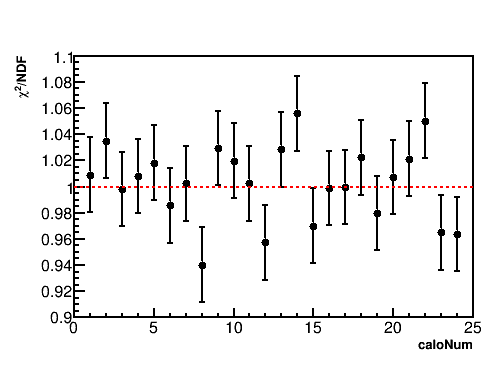
\includegraphics[width=\textwidth]{FullRatioFit_Chi2NDF_Vs_Calo_Canv_Endgame}
%         \caption{Endgame dataset.}
%     \end{subfigure}
% \caption[\chisq/NDF versus calorimeter number]{\chisq/NDF versus calorimter for the Run~1 precession frequency analysis datasets.}
% \label{fig:caloFits_chi2}
% \end{figure}

% \begin{figure}[]
% \centering
%     \begin{subfigure}[]{0.45\textwidth}
%         \centering
%         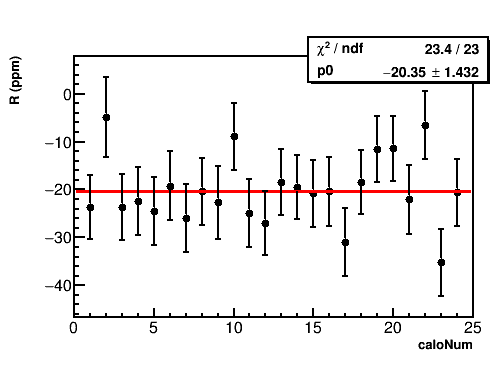
\includegraphics[width=\textwidth]{FullRatioFit_R_Vs_Calo_Canv_60h}
%         \caption{60h dataset.}
%     \end{subfigure}% %you need this % here to add spacing between subfigures
%     \begin{subfigure}[]{0.45\textwidth}
%         \centering
%         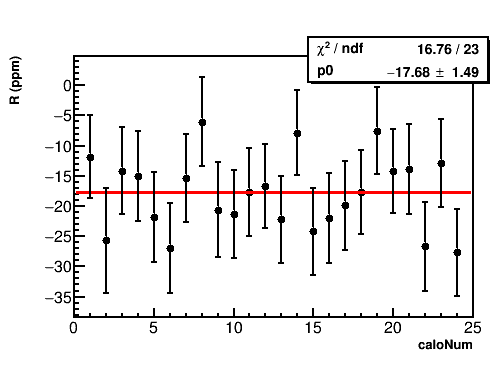
\includegraphics[width=\textwidth]{FullRatioFit_R_Vs_Calo_Canv_HighKick}
%         \caption{HighKick dataset.}
%     \end{subfigure}

%     \begin{subfigure}[]{0.45\textwidth}
%         \centering
%         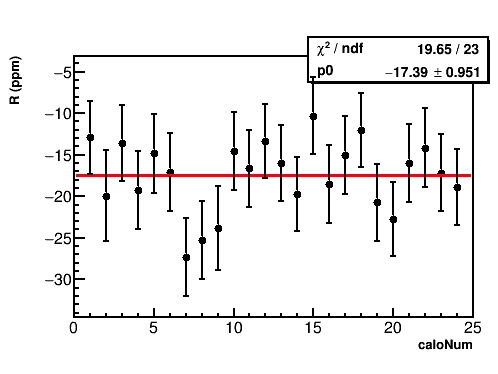
\includegraphics[width=\textwidth]{FullRatioFit_R_Vs_Calo_Canv_9d}
%         \caption{9d dataset.}
%     \end{subfigure}% %you need this % here to add spacing between subfigures
%     \begin{subfigure}[]{0.45\textwidth}
%         \centering
%         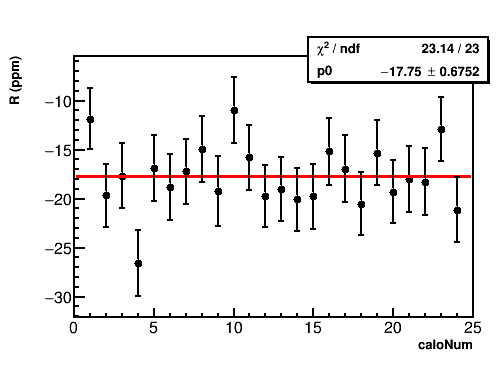
\includegraphics[width=\textwidth]{FullRatioFit_R_Vs_Calo_Canv_Endgame}
%         \caption{Endgame dataset.}
%     \end{subfigure}
% \caption[$R$ versus calorimeter number]{$R$ versus calorimter for the Run~1 precession frequency analysis datasets. A straight line fit was performed on the fitted values, with the fit result shown in the upper right box as parameter $p_{1}$ in units of ppm.}
% \label{fig:caloFits_R}
% \end{figure}
